\chapter{Selbstevaluation}\label{cha:theoretical-background}
\section{Probleme bei der Entwicklung}
\subsection{Event-Handling mit MVVM-Light}
Als Alternative zu den vielen einzelnen Fenstern für das Anlegen und Bearbeiten von Daten, wäre am Anfang eigentlich geplant gewesen, Datagrids zu benutzen. Ein Datagrid ist vergleichbar mit einer Excel-Tabelle. Das bedeutet, dass es vordefinierte Spalten gibt und die Daten in einer Tabelle darunter angezeigt werden. 
\begin{figure}[H]
\begin{center}
	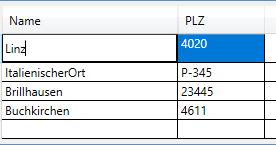
\includegraphics[scale=.75]{images/datagrid.png}
\end{center}
	\caption{Screenshot eines DataGrids}
	\label{fig:sample}
\end{figure}
\noindent Während des Entwickelns des Programmes mit DataGrids sind allerdings einige Fragen aufgekommen. Die wichtigste war: Wann werden die Daten überprüft und in die Datenbank gespeichert? Die sinnvollste Antwort auf diese Frage wäre gewesen: Nachdem der Benutzer das Feld verlässt. Allerdings wäre dazu das Abonnieren eines Events aus der View ('RowEditEnding') mittels EventToCommand von MVVM-Light notwendig gewesen, doch das war auch nach unzähligen Lösungsversuchen aus unerklärlichen Gründen nicht möglich. Grundsätzlich gibt es zwei Möglichkeiten, um Events aus der View abzufangen:
\begin{itemize}
\item Events mittels Mouse- und KeyBindings auf Commands in das ViewModel übertragen. Für Events für Maus und Tastatur ist das eine sehr praktische Lösungsmöglichkeit, allerdings können damit keine anderen Events behandelt werden.
\item Alle Events mittels MVVM-Light und der EventToCommand-Funktion ins ViewModel übertragen (Kapitel 2.5).
\end{itemize}
Das 'RowEditEnding'-Event fällt leider in die zweite Kategorie, weshalb es nicht möglich war dieses Event zu behandeln. Als Alternative wurde versucht, die Daten erst nach dem Drücken der Enter-Taste in die Datenbank zu speichern. Das wäre möglich gewesen, weil dann auf ein Event der Tastatur mittels KeyBinding reagiert werden hätte können. Doch auch diese Variante war nicht optimal, denn sobald der Benutzer einmal vergessen hätte die Enter-Taste zu betätigen, wären die Daten nicht gesichert gewesen. Aus diesem Grund wurde dann ein ganz anderer Ansatz gewählt, nämlich der der ListViews. Damit konnte das Problem des Event-Handlings umgangen werden und diese Variante ist auch benutzerfreundlicher. So öffnet sich nun zum Anlegen sowie zum Bearbeiten eines Datensatzes ein neues Fenster. \newline In der späteren Entwicklungsphase haben sich die Probleme mit MVVM-Light und EventToCommand dann aus unerfindlichen Gründen gelöst und somit konnten alle Events verwendet werden. Das war insbesondere zum Sortieren wichtig (Kapitel 3.1.8). Dennoch blieb man aber bei der Variante der neuen Fenster für das Bearbeiten und Anlegen von Daten, da es sich als viel benutzerfreundlicher erwies.
\subsection{UnitOfWork-Instanzen}
In der frühen Entwicklungsphase der Diplomarbeit traten Probleme mit dem Speichern der Daten in der Datenbank auf. Auf unerklärliche Weise wurden veränderte Daten schon vor dem eigentlichen Speichern in der UnitOfWork-Instanz geändert und somit konnten Veränderungen nie rückgängig gemacht werden. \newline Beispiel: Der Benutzer öffnet einen Kunden und möchte den Vornamen von 'Max' auf 'Maxi' ändern. Bevor er die Änderung speichert, beschließt er allerdings, dass er die Änderung doch nicht vornehmen möchte und klickt statt 'Speichern' auf 'Abbrechen'. Wenn er nun zurück auf der Startseite ist, wurde der Vorname aber trotzdem auf 'Maxi' geändert. \newline Später stellte sich heraus, dass der Grund dafür war, dass im Programm nur eine UnitOfWork-Instanz verwendet wurde und immer nur mit Referenzen von Objekten in der UnitOfWork-Instanz gearbeitet wurde. Lösungen für das Problem wären gewesen für jeden Datenbankzugriff eine neue UnitOfWork-Instanz zu erzeugen oder alle Daten, die veränderbar sein sollten, vorher lokal kopiert. Schlussendlich wurde entschieden weiterhin nur eine UnitOfWork-Instanz zu verwenden und alle veränderbaren Daten vorher lokal zu kopieren. Die andere Möglichkeit, bei der für jeden Datenbankzugriff eine neue UnitOfWork-Instanz erzeugt worden wäre, hätte den Code um einiges verlängert und unübersichtlicher gemacht. Dazu hätte für jeden Zugriff ein Using-Block verwendet werden müssen:  
\begin{lstlisting}
using(UnitOfWork uow = new UnitOfWork())
{
	Customer cus = uow.CustomerRepository.GetById(1);
}
\end{lstlisting}